\documentclass[aspectratio=169]{beamer}



\mode<presentation>
{
 \usetheme[reversetitle,notitle,noauthor]{Wien}
%    \usetheme[noauthor]{Wien}
}

\usepackage{url}
\usepackage{graphicx}
\graphicspath{{./}{./Figures/}}

\usepackage{appendixnumberbeamer}
\usepackage{algorithm2e}
\usepackage{float}
\usepackage{tikz}
\usetikzlibrary{arrows.meta,positioning}
\usetikzlibrary{positioning}
\usetikzlibrary{overlay-beamer-styles}

\tikzset{onslide/.code args={<#1>#2}{%
  \only<#1>{\pgfkeysalso{#2}} % \pgfkeysalso doesn't change the path
}}
\tikzset{temporal/.code args={<#1>#2#3#4}{%
  \temporal<#1>{\pgfkeysalso{#2}}{\pgfkeysalso{#3}}{\pgfkeysalso{#4}} % \pgfkeysalso doesn't change the path
}}

\tikzstyle{highlight}=[red,ultra thick]

% To avoid a warning from the hyperref package:
\pdfstringdefDisableCommands{%
    \def\translate{}%
}

% To make sure, that the footnote is placed above and outside the
% footline (but it only works for one footnote per frame):
%
% \addtobeamertemplate{footnote}{}{\vspace{4ex}}

%%%%%%%%%%%%%%%%%%%%%%%%%%%%%%%%%%%%%%%%%%%%%%%%%%%%%%%%%%%%%%%%%%%%%%%%%%%%%
%%%%%%%%%%%%%%%%%%%%%%%%%%%%%%%%%%%%%%%%%%%%%%%%%%%%%%%%%%%%%%%%%%%%%%%%%%%%%
\title[Zelluläre Automaten]{Design und Analyse eines Spiels \newline mithilfe von Zellulären Automaten}


\subtitle{Bachelorarbeit aus Diskreter Mathematik}

\author[C. Göth]{Christian Göth}

\institute[TU Wien]{TU Wien, Vienna, Austria}

\date{26. April 2021}

% Hier befinden sich Pakete, die wir beinahe immer benutzen ...

\usepackage[utf8]{inputenc}

% Sprach-Paket:
\usepackage[ngerman]{babel}

% damit's nicht so, wie beim Grill aussieht:
\usepackage{fullpage}

% Mathematik:
\usepackage{amsmath, amssymb, amsfonts, amsthm}
\usepackage{bbm}
\usepackage{mathtools, mathdots}

% Makros mit mehereren Default-Argumenten:
\usepackage{twoopt}

% Anführungszeichen (Makro \Quote{}):
\usepackage{babel}

% if's für Makros:
\usepackage{xifthen}
\usepackage{etoolbox}

% tikz ist kein Zeichenprogramm (doch!):
\usepackage{tikz}

% bessere Aufzählungen:
\usepackage{enumitem}

% (bessere) Umgebung für Bilder:
\usepackage{graphicx, subfig, float}

% Umgebung für Code:
\usepackage{listings}

% Farben:
\usepackage{xcolor}

% Umgebung für "plain text":
\usepackage{verbatim}

% Umgebung für mehrerer Spalten:
\usepackage{multicol}

% "nette" Brüche
\usepackage{nicefrac}

% Spaltentypen verschiedener Dicke
\usepackage{tabularx}
\usepackage{makecell}

% Für Vektoren
\usepackage{esvect}

% (Web-)Links
\usepackage{hyperref}

% Zitieren & Literatur-Verzeichnis
\usepackage[style = authoryear]{biblatex}
\usepackage{csquotes}

% so ähnlich wie mathbb
%\usepackage{mathds}

% Keine Ahnung, was das macht ...
\usepackage{booktabs}
\usepackage{ngerman}
\usepackage{placeins}

% special letters:

\newcommand{\N}{\mathbb{N}}
\newcommand{\Z}{\mathbb{Z}}
\newcommand{\Q}{\mathbb{Q}}
\newcommand{\R}{\mathbb{R}}
\newcommand{\C}{\mathbb{C}}
\newcommand{\K}{\mathbb{K}}
\newcommand{\T}{\mathbb{T}}
\newcommand{\E}{\mathbb{E}}
\newcommand{\V}{\mathbb{V}}
\renewcommand{\S}{\mathbb{S}}
\renewcommand{\P}{\mathbb{P}}
\newcommand{\1}{\mathbbm{1}}

% quantors:

\newcommand{\Forall}{\forall \,}
\newcommand{\Exists}{\exists \,}
\newcommand{\ExistsOnlyOne}{\exists! \,}
\newcommand{\nExists}{\nexists \,}
\newcommand{\ForAlmostAll}{\forall^\infty \,}

% MISC symbols:

\newcommand{\landau}{{\scriptstyle \mathcal{O}}}
\newcommand{\Landau}{\mathcal{O}}


\newcommand{\eps}{\mathrm{eps}}

% graphics in a box:

\newcommandtwoopt
{\includegraphicsboxed}[3][][]
{
  \begin{figure}[!h]
    \begin{boxedin}
      \ifthenelse{\isempty{#1}}
      {
        \begin{center}
          \includegraphics[width = 0.75 \textwidth]{#3}
          \label{fig:#2}
        \end{center}
      }{
        \begin{center}
          \includegraphics[width = 0.75 \textwidth]{#3}
          \caption{#1}
          \label{fig:#2}
        \end{center}
      }
    \end{boxedin}
  \end{figure}
}

% braces:

\newcommand{\pbraces}[1]{{\left  ( #1 \right  )}}
\newcommand{\bbraces}[1]{{\left  [ #1 \right  ]}}
\newcommand{\Bbraces}[1]{{\left \{ #1 \right \}}}
\newcommand{\vbraces}[1]{{\left  | #1 \right  |}}
\newcommand{\Vbraces}[1]{{\left \| #1 \right \|}}
\newcommand{\abraces}[1]{{\left \langle #1 \right \rangle}}
\newcommand{\round}[1]{\bbraces{#1}}

\newcommand
{\floorbraces}[1]
{{\left \lfloor #1 \right \rfloor}}

\newcommand
{\ceilbraces} [1]
{{\left \lceil  #1 \right \rceil }}

% special functions:

\newcommand{\norm}  [2][]{\Vbraces{#2}_{#1}}
\newcommand{\diam}  [2][]{\mathrm{diam}_{#1} \: #2}
\newcommand{\diag}  [1]{\mathrm{diag} \: #1}
\newcommand{\dist}  [1]{\mathrm{dist} \: #1}
\newcommand{\mean}  [1]{\mathrm{mean} \: #1}
\newcommand{\erf}   [1]{\mathrm{erf} \: #1}
\newcommand{\id}    [1]{\mathrm{id} \: #1}
\newcommand{\sgn}   [1]{\mathrm{sgn} \: #1}
\newcommand{\supp}  [1]{\mathrm{supp} \: #1}
\newcommand{\arsinh}[1]{\mathrm{arsinh} \: #1}
\newcommand{\arcosh}[1]{\mathrm{arcosh} \: #1}
\newcommand{\artanh}[1]{\mathrm{artanh} \: #1}
\newcommand{\card}  [1]{\mathrm{card} \: #1}
\newcommand{\Span}  [1]{\mathrm{span} \: #1}
\newcommand{\Aut}   [1]{\mathrm{Aut} \: #1}
\newcommand{\End}   [1]{\mathrm{End} \: #1}
\newcommand{\ggT}   [1]{\mathrm{ggT} \: #1}
\newcommand{\kgV}   [1]{\mathrm{kgV} \: #1}
\newcommand{\ord}   [1]{\mathrm{ord} \: #1}
\newcommand{\grad}  [1]{\mathrm{grad} \: #1}
\newcommand{\ran}   [1]{\mathrm{ran} \: #1}
\newcommand{\graph} [1]{\mathrm{graph} \: #1}
\newcommand{\Inv}   [1]{\mathrm{Inv} \: #1}
\newcommand{\pv}    [1]{\mathrm{pv} \: #1}
\newcommand{\GL}    [1]{\mathrm{GL} \: #1}
\newcommand{\Mod}{\mathrm{Mod} \:}
\newcommand{\Th}{\mathrm{Th} \:}
\newcommand{\Char}{\mathrm{char}}
\newcommand{\At}{\mathrm{At}}
\newcommand{\Ob}{\mathrm{Ob}}
\newcommand{\Hom}{\mathrm{Hom}}
\newcommand{\orthogonal}[3][]{#2 ~\bot_{#1}~ #3}
\newcommand{\Rang}{\mathrm{Rang}}
\newcommand{\NIL}{\mathrm{NIL}}
\newcommand{\Res}{\mathrm{Res}}
\newcommand{\lxor}{\dot \lor}
\newcommand{\Div}{\mathrm{div} \:}
\newcommand{\meas}{\mathrm{meas} \:}

% fractions:

\newcommand{\Frac}[2]{\frac{1}{#1} \pbraces{#2}}
\newcommand{\nfrac}[2]{\nicefrac{#1}{#2}}

% derivatives & integrals:

\newcommandtwoopt
{\Int}[4][][]
{\int_{#1}^{#2} #3 ~\mathrm{d} #4}

\newcommandtwoopt
{\derivative}[3][][]
{
  \frac
  {\mathrm{d}^{#1} #2}
  {\mathrm{d} #3^{#1}}
}

\newcommandtwoopt
{\pderivative}[3][][]
{
  \frac
  {\partial^{#1} #2}
  {\partial #3^{#1}}
}

\newcommand
{\primeprime}
{{\prime \prime}}

\newcommand
{\primeprimeprime}
{{\prime \prime \prime}}

% Text:

\newcommand{\Quote}[1]{\glqq #1\grqq{}}
\newcommand{\Text}[1]{{\text{#1}}}
\newcommand{\fastueberall}{\text{f.ü.}}
\newcommand{\fastsicher}{\text{f.s.}}

\theoremstyle{definition}

% unnumbered theorems
\newtheorem*{theorem*}    {Satz}
\newtheorem*{lemma*}      {Lemma}
\newtheorem*{corollary*}  {Korollar}
\newtheorem*{proposition*}{Proposition}
\newtheorem*{remark*}     {Bemerkung}
\newtheorem*{definition*} {Definition}
\newtheorem*{example*}    {Beispiel}
\newtheorem*{problem*}    {Problem}
\newtheorem*{algorithmus*}    {Algorithmus}
\newtheorem*{algorithmen*}    {Weiterführende Algorithmen}
\newtheorem*{anwendungen*}    {Anwendungen}

\renewcommand{\figurename}{Abbildung}
\renewcommand{\tablename} {Tabelle}


\begin{document}

\begin{frame}
    \titlepage
\end{frame}

%%%%%%%%%%%%%%%%%%%%%%%%%%%%%%%%%%%%%%%%%%%%%%%%%%%%%%%%%%%%%%%%%%%%%%%%%%%%%
%%%%%%%%%%%%%%%%%%%%%%%%%%%%%%%%%%%%%%%%%%%%%%%%%%%%%%%%%%%%%%%%%%%%%%%%%%%%%
%%%%%%%%%%%%%%%%%%%%%%%%%%%%%%%%%%%%%%%%%%%%%%%%%%%%%%%%%%%%%%%%%%%%%%%%%%%%%


  \begin{frame}{Einleitung}

    \begin{block}{Zelluläre Automaten}
      \begin{itemize}
        \item Erstmals um 1940 durch John von Neumann erforscht \\ %%vorgestellt von Stanislaw Ulam
        \item Sind zeitlich diskret \\
        \item Sind räumlich diskret \\
        \item Geeignet zur Simulation komplexer physikalischer oder biologischer Systeme
      \end{itemize}
    \end{block}

  \end{frame}



  \begin{frame}{Wohl bekanntester zellulärer Automat}
    \begin{block}{"Game of Life"}
      \begin{itemize}
        \item Zweidimensionaler zellulärer Automat
        \item Von John Horton Conway 1970 entworfen %%eineinhalb Jahre mit Kollegen experimentiert, ohne Computer-Unterstützung
        \item Veröffentlichung in Scientific American %%erfreute sich großer Beliebtheit, Hype um Challenge
        \item Komplexes Verhalten aus einfachen Regeln
      \end{itemize}
    \end{block}

    \pause

    \begin{block}{Satz [Berlekamp et al.]}
      \textit{Game of Life is computationally universal. It is undecidable whether a given finite configuration dies.}
    \end{block}

  \end{frame}


  \begin{frame}{Regeln des Game of Life}

    \begin{enumerate}
      \item Eine lebendige Zelle mit weniger als 2 oder mehr als 3 lebendigen Nachbarn stirbt %%Unterpopulation oder Überpopulation
      \item Eine tote Zelle mit genau 3 lebendigen Nachbarn wird lebendig %%Reproduktion
      \item Alle anderen Zellen behalten ihren Zustand
    \end{enumerate}

    \pause

    \begin{multicols*}{3}

      \begin{figure}[H]
          \centering
          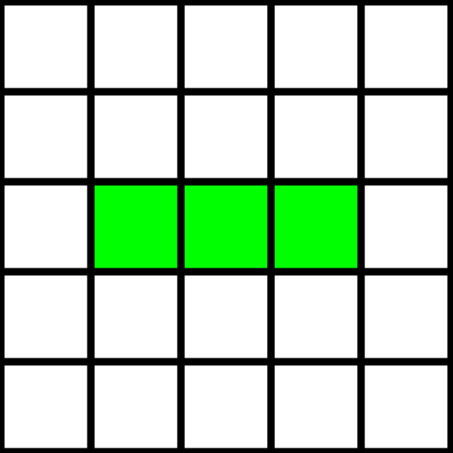
\includegraphics[height = 0.3 \textheight]{start_oscillator.png}
      \end{figure}
      \centering{$t = 0$}

      \pause

      \begin{figure}[H]
          \centering
          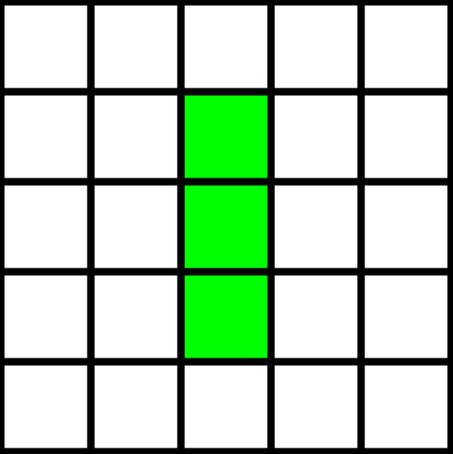
\includegraphics[height = 0.3 \textheight]{end_oscillator.png}
      \end{figure}
      \centering{$t = 1$}

      \pause

      \begin{figure}[H]
          \centering
          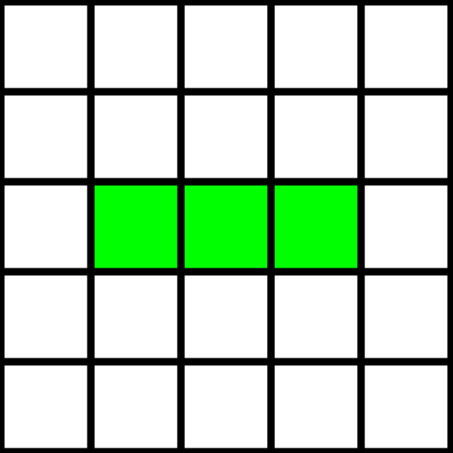
\includegraphics[height = 0.3 \textheight]{start_oscillator.png}
      \end{figure}
      \centering{$t = 2$}

    \end{multicols*}
    %%Erinnerung - alle Updates simultan

  \end{frame}

  \begin{frame}{Definitionen 1/5}
    \begin{definition*}[Zellularraum]
      Für $d \in \mathbb{N}$ betrachten wir ein $d$-dimensionales unendliches Gitter, dessen \textit{Zellen} mit Elementen aus $\mathbb{Z}^d$ identifiziert werden.
    \end{definition*}

    \begin{multicols*}{3}
      \centering{$d = 1$}
      \begin{figure}[H]
          \centering
          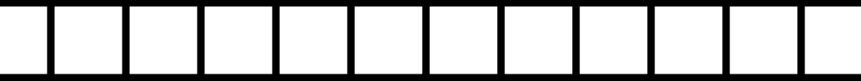
\includegraphics[width = 0.4 \textheight]{1d_cellspace.png}
      \end{figure}
      \vfill\null
      \columnbreak

      \pause

      \centering{$d = 2$}
      \begin{figure}[H]
          \centering
          
\includegraphics[width = 0.35 \textheight]{2d_cellspace.png}
      \end{figure}
      \vfill\null
      \columnbreak

      \pause

      \centering{$d = 3$}
      \begin{figure}[H]
          \centering
          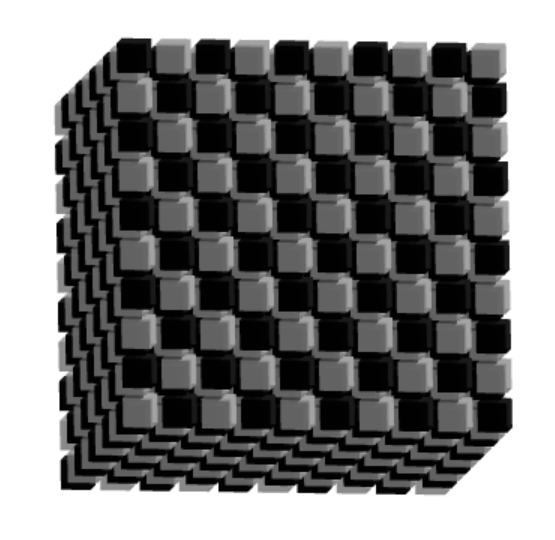
\includegraphics[width = 0.35 \textheight]{3d_cellspace.png}
      \end{figure}


    \end{multicols*}

  \end{frame}



  \begin{frame}{Definitionen 2/5}
    \begin{definition*}
      Sei $S$ eine endliche \textit{Zustandsmenge}. Eine Abbildung $c: \mathbb{Z}^d \to S$  heißt $Konfiguration$. \\
      Die Menge $S^{\mathbb{Z}^d}$ aller Konfigurationen bezeichnen wir mit $\mathcal{C}(d, S) = \mathcal{C}$.
    \end{definition*}

    \pause

    Beispiel für $S = \{0, 1\}$:
    \begin{figure}[H]
        \centering
        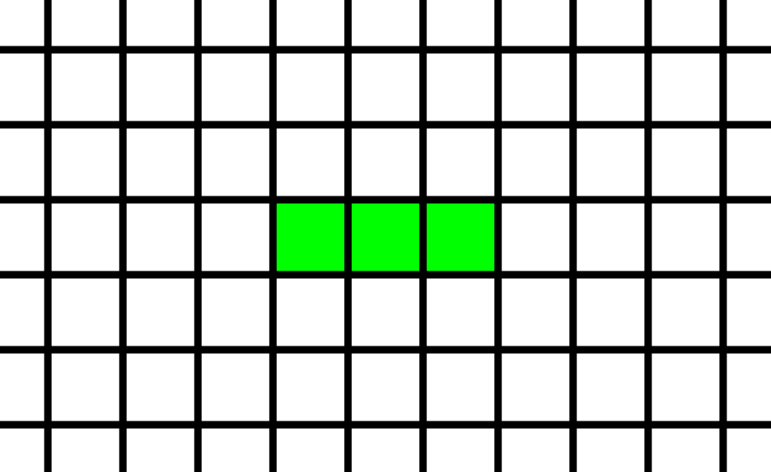
\includegraphics[width = 0.35 \textheight]{configuration.png}
    \end{figure}

  \end{frame}


  \begin{frame}{Definitionen 3/5}
    \begin{definition*}[Nachbarschaft]
      Wir bezeichnen einen Vektor $N = (y_1, y_2, \dots, y_n)$ aus $n$ paarweise verschiedenen Elementen aus $\mathbb{Z}^d$ als \textit{Nachbarschaft}. Die \textit{Nachbarn} einer beliebigen Zelle $x \in \mathbb{Z}^d$ sind dann genau die Zellen $(x + y_1, x + y_2, \dots, x + y_n)$.
    \end{definition*}

    \pause

    Beispiele bekannter Nachbarschaften:

    \begin{multicols*}{2}
      \begin{multicols*}{2}
        \begin{figure}[H]
          \centering
          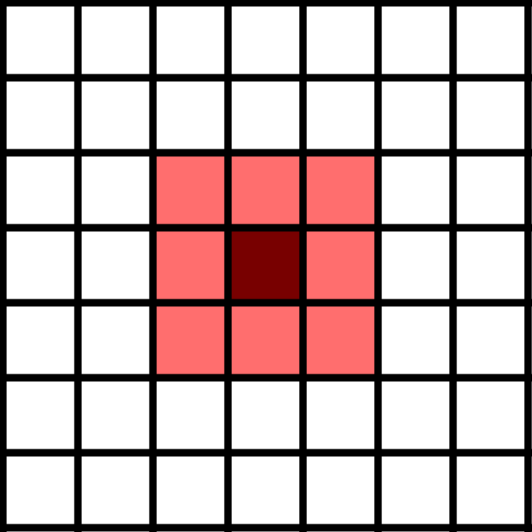
\includegraphics[width = 0.28 \textheight]{moore_1.png}
        \end{figure}

        \begin{figure}[H]
          \centering
          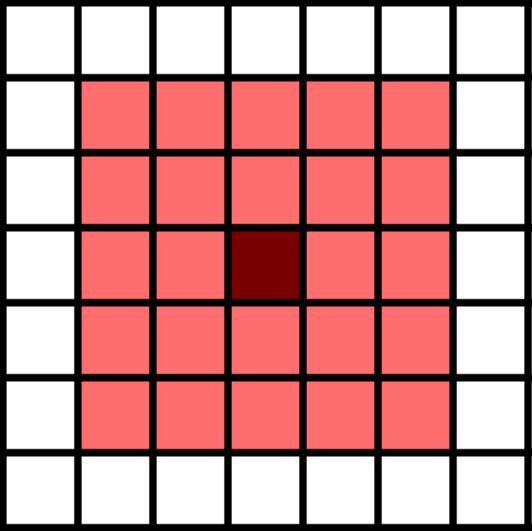
\includegraphics[width = 0.28 \textheight]{moore_2.png}
        \end{figure}

      \end{multicols*}

      \centering{Moore - $N = (y: \|y\|_{\infty} \leq r)$}

      \vfill\null

      \pause


      \begin{multicols*}{2}
      \begin{figure}[H]
        \centering
        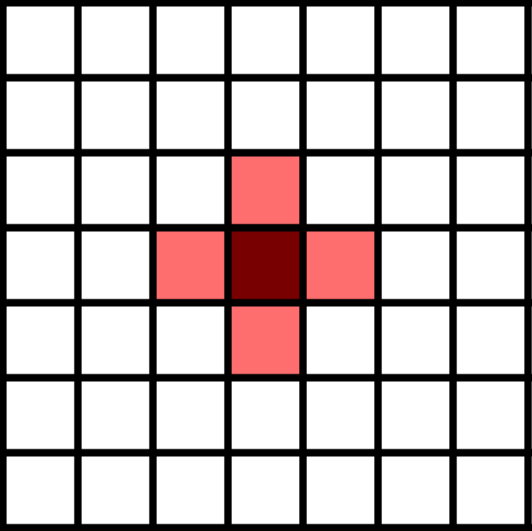
\includegraphics[width = 0.28 \textheight]{von_Neumann_1.png}
      \end{figure}

      \begin{figure}[H]
        \centering
        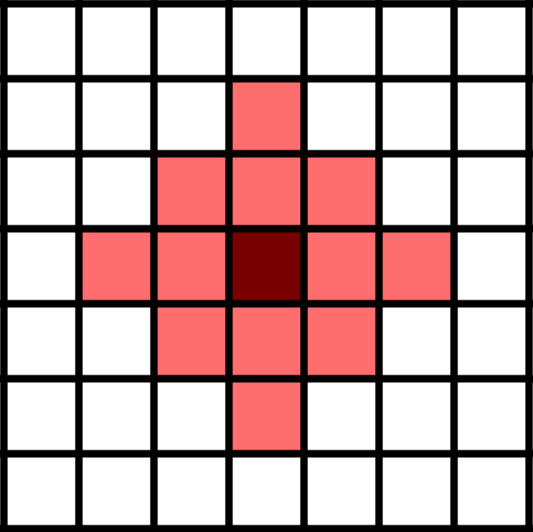
\includegraphics[width = 0.28 \textheight]{von_Neumann_2.png}
      \end{figure}

      \end{multicols*}

      \centering{von Neumann - $N = (y: \|y\|_1 \leq r)$}

      \vfill\null

    \end{multicols*}

  \end{frame}



  \begin{frame}{Nachbarschaften am Rand}


    \begin{multicols*}{5}

      \onslide<2->\begin{figure}[H]
        \centering
        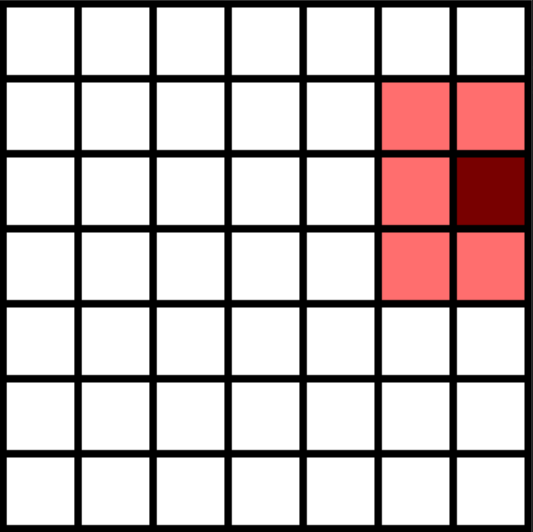
\includegraphics[width = 0.25 \textheight]{neighborhood_border_sol1.png}
      \end{figure}

      \vfill\null

      \onslide<2->\centering{\Huge $\leftarrow$ \par}
      \vfill\null

      \onslide<1->\begin{figure}[H]
        \centering
        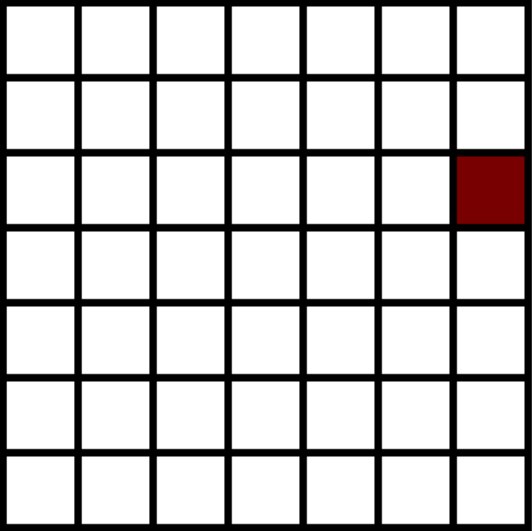
\includegraphics[width = 0.25 \textheight]{neighborhood_border.png}
      \end{figure}

      \vfill\null



      \onslide<3->\centering{\Huge $\rightarrow$ \par}
      \vfill\null

      \onslide<3->\begin{figure}[H]
        \centering
        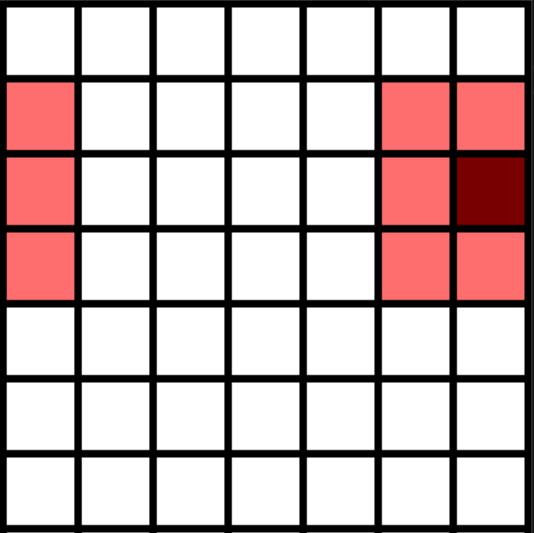
\includegraphics[width = 0.25 \textheight]{neighborhood_border_sol2.png}
      \end{figure}

    \end{multicols*}

    \onslide<4->\begin{multicols*}{5}
      \vfill\null
      \vfill\null
      \vfill\null
      \vfill\null
      \vfill\null
      \vfill\null
      \vfill\null
      \vfill\null
      \vfill\null
      \vfill\null
      \vfill\null

      \centering{\Huge $\Downarrow$ \par}

      \vfill\null


    \end{multicols*}

    \begin{multicols*}{4}
      \vfill\null
      \vfill\null
      \vfill\null
      \vfill\null
      \vfill\null
      \vfill\null
      \vfill\null
      \vfill\null
      \vfill\null
      \vfill\null

      \begin{figure}[H]
        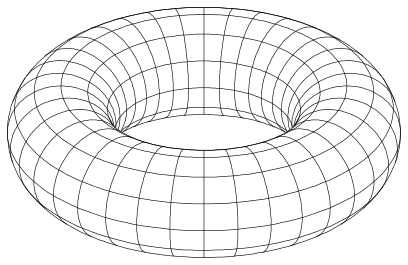
\includegraphics[width = 0.35 \textheight]{torus.png}
      \end{figure}

    \end{multicols*}

  \end{frame}



    \begin{frame}{Definitionen 4/5}
      \begin{definition*}[Lokale Update-Regel]
        Sei $n$ die Größe der Nachbarschaft. Die \textit{Lokale Update-Regel} ist eine Funktion $f: S^n \to S$, die für jede Zelle $x \in \mathbb{Z}^d$ ihren neuen Zustand bestimmt, abhängig von den Zuständen der $n$ Nachbarn zum vorherigen Zeitschritt.
      \end{definition*}

      \pause

      Eine Konfiguration $c \in \mathcal{C}$ wird also im nächsten Zeitschritt zu der Konfiguration $e \in \mathcal{C}$, die gegeben ist durch
      \begin{align}\label{ctoe}
        e(x) = f \big(c(x+y_1), c(x+y_2), \dots, c(x+y_n)\big).
      \end{align}

      \pause

      \begin{definition*}[Globale Überführungsfunktion]
        Die Funktion $G: \mathcal{C} \to \mathcal{C}$, die $G(c)=e$ gemäß \eqref{ctoe} erfüllt, nennen wir \textit{Globale Überführungsfunktion}.
      \end{definition*}

    \end{frame}



  \begin{frame}{Definitionen 5/5}
    \begin{definition*}[Zellulärer Automat]
      In $\mathbb{Z}^d$ ist ein \textit{$d$-dimensionaler Zellulärer Automat (ZA)} gegeben durch das Tripel $(S,N,f)$, wobei $S$ die Zustandsmenge, $N$ die Nachbarschaft und $f$ die Lokale Update-Regel bezeichnen.
    \end{definition*}

    \pause

    \begin{remark*}
      Wir identifizieren einen ZA auch durch seine Globale Überführungsfunktion $G$, welche ebenso durch das Tripel $(S,N,f)$ bestimmt ist, und sprechen vom ZA $G$.
    \end{remark*}

  \end{frame}



  \begin{frame}{Beispiele}

    \begin{example*}
      Seien $G_1$ und $G_2$ zwei ZA mit gleicher Zustandsmenge und Dimension. Die \textit{Komposition} $G_1 \circ G_2$ ist wiederum ein ZA mit Nachbarschaft $N_1 + N_2$.

      Falls $G_1 \circ G_2 = G_2 \circ G_1 = id$ gilt, so nennen wir $G_1$ und $G_2$ \textit{reversibel}.
    \end{example*}

    \pause

    \begin{example*}
      Für einen ZA G nennen wir die Konfiguration $c \in \mathcal{C}$ \textit{zeitlich periodisch}, wenn $G^k(c) = c$ für ein $k \geq 1$. Für $k= 1$ nennen wir $c$ Fixpunkt von $G$.
    \end{example*}

  \end{frame}



  \begin{frame}{Ausblick}
    \begin{block}{Design des Spiels}
      \begin{itemize}
        \item Implementierung in Python
        \item 2-dimensionales Gitter
        \item Voraussichtlich 1 oder 2 Spieler
        \item Erweiterung auf stochastische Update-Regel
      \end{itemize}
    \end{block}

    \pause

    \begin{block}{Analyse des Spiels}
      \begin{itemize}
        \item Abhängig, ob stochastisch oder deterministisch
        \item Zeitreihenanalyse
        \item Entscheidbarkeit
        \item Reversibilität
        \item Periodizität, Grenzzyklen
      \end{itemize}

    \end{block}


  \end{frame}



  \begin{frame}{}
    \begin{block}{}

      {
          \centering
          \huge
          Präsentation der Ergebnisse am 21. Juni 2021.
      }

    \end{block}

  \end{frame}


\end{document}


%%% Local Variables:
%%% mode: latex
%%% TeX-master: t
%%% End:
